\let\lesson\undefined
\newcommand{\lesson}{\phantomlesson{Bài 12: Một số lực trong thực tiễn}}
\chapter[Lực ma sát]{Lực ma sát}
\setcounter{section}{0}
\section{Lý thuyết}
\subsection{Lực ma sát nghỉ}
\subsubsection{Định nghĩa}
Lực ma sát nghỉ xuất hiện ở mặt tiếp xúc khi một vật nằm yên trên bề mặt vật khác và có xu hướng chuyển động dưới tác dụng của ngoại lực.
\begin{center}
	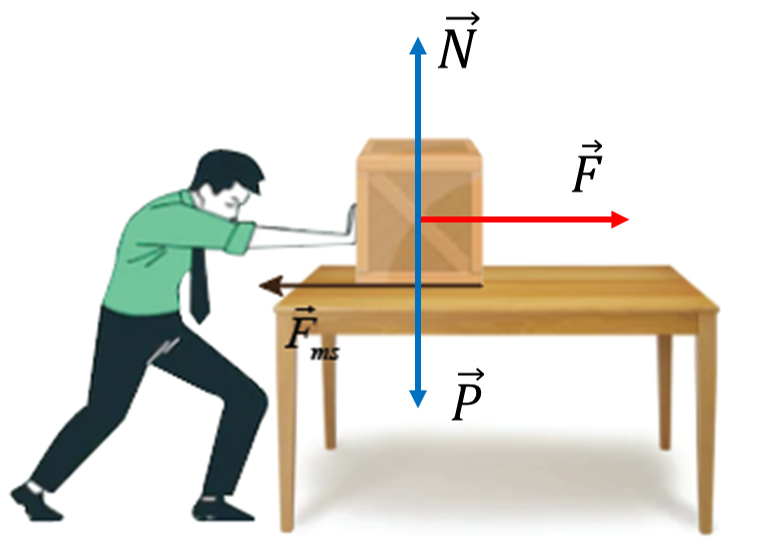
\includegraphics[width=0.4\linewidth]{../figs/VN10-2023-PH-TP019-1}
	\captionof{figure}{Thùng gỗ bất động khi bị người đẩy.}
\end{center}
\subsubsection{Đặc điểm}
\begin{itemize} 
	\item Điểm đặt: trên vật và ngay tại vị trí tiếp xúc của hai bề mặt, 
	\item Phương: tiếp tuyến với bề mặt tiếp xúc,
	\item Chiều: ngược chiều xu hướng chuyển động tương đối của hai bề mặt tiếp xúc,
	\item Độ lớn: bằng độ lớn của lực tác dụng gây ra xu hướng chuyển động.
\end{itemize}
\luuy{Điều kiện để vật trượt 
$$F\ge F_{msn\ \text{max}}=\mu_N\cdot N$$
trong đó:
\begin{itemize}
	\item $F_{msn\ \text{max}}$: lực ma sát nghỉ cực đại;
	\item $\mu_N$: hệ số ma sát nghỉ;
	\item $N$: áp lực do vật tác dụng lên bề mặt tiếp xúc.
\end{itemize}
Lực ma sát nghỉ cực đại lớn hơn ma sát trượt.
}
\subsection{Lực ma sát trượt}
\subsubsection{Định nghĩa}
Lực ma sát trượt xuất hiện ở mặt tiếp xúc khi một vật trượt trên một bề mặt và cản trở lại chuyển động trượt của vật đó.
\begin{center}
	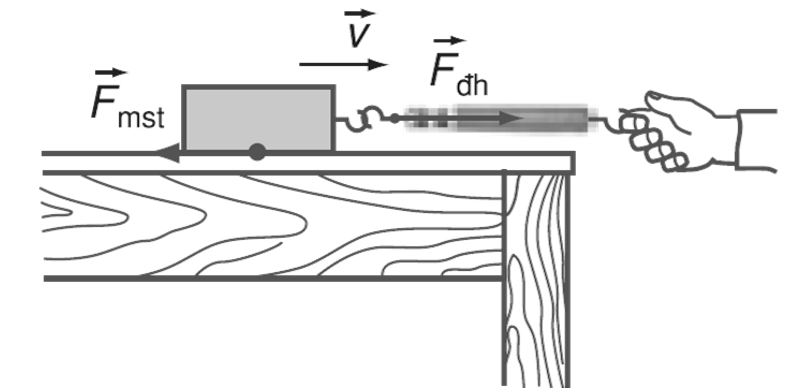
\includegraphics[scale=0.35]{../figs/VN10-PH-15-L-012-1-V2-01.JPG}
\end{center}
\subsubsection{Đặc điểm}
\begin{itemize}
	\item Điểm đặt: trên vật và ngay tại vị trí tiếp xúc của hai bề mặt,
	\item Phương: tiếp tuyến với mặt tiếp xúc giữa 2 vật trượt,
	\item Chiều: ngược chiều với vận tốc tương đối của vật ấy đối với vật kia,
	\item Độ lớn:
	\begin{itemize}
		\item không phụ thuộc vào diện tích tiếp xúc và tốc độ của vật.
		\item tỉ lệ với độ lớn của áp lực.
		\item phụ thuộc vào vật liệu và tình trạng của hai mặt tiếp xúc.
	\end{itemize}
	\item Biểu thức 
	\begin{equation*}
		F_{\text{mst}} = \mu_{\text{t}} \cdot N,
	\end{equation*}
	trong đó:
	
	+ $\mu_{\text{t}}$ là hệ số ma sát trượt, nó phụ thuộc vào bản chất của hai mặt tiếp xúc và các điều kiện trên bề mặt (không có đơn vị),
	
	+ $N$ là áp lực của vật lên mặt tiếp xúc.
\end{itemize}
\subsubsection{Vai trò}
\begin{itemize}
	\item Ma sát trượt có ích trong việc mài dũa, thắng xe, \dots
	\item Ma sát trượt có hại trong các ổ trục trượt, mài mòn xilanh, pittông xe, \dots Để giảm ma sát trượt, người ta bôi trơn các chi tiết bằng dầu mỡ công nghiệp.
\end{itemize}
\subsection{Lực ma sát lăn}
\begin{itemize}
	\item Lực ma sát lăn xuất hiện ở mặt tiếp xúc khi một vật lăn trên một bề mặt và cản trở lại chuyển động lăn của vật đó.
	\item Lực ma sát lăn có các đặc điểm giống như lực ma sát trượt nhưng hệ số ma sát lăn nhỏ hơn rất nhiều lần (hàng chục lần) hệ số ma sát trượt.
	\item Trong trường hợp lực ma sát trượt có hại, cần phải giảm thì người ta dùng con lăn hay ổ bi đặt xen vào giữa hai mặt tiếp xúc để giảm tổn hại vì ma sát.
\end{itemize}
\begin{center}
	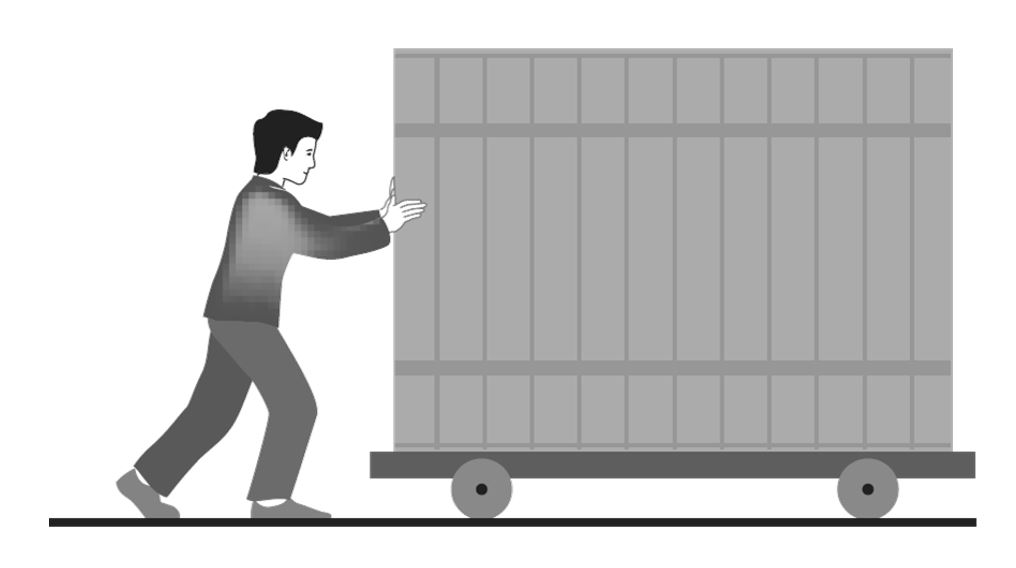
\includegraphics[scale=0.25]{../figs/VN10-PH-15-L-012-1-V2-02.JPG}
\end{center}

\subsubsection{Vai trò}
\begin{itemize}
	\item Giúp ta cầm nắm được các vật, giữ vật ở yên tại vị trí đã định, dây cua roa truyền được chuyển động giữa các bánh xe, băng chuyền vận chuyển được người hoặc vật từ nơi này đến nơi khác...
	\item Đóng vai trò lực phát động, giúp sinh vật, xe cộ di chuyển được.
	\begin{center}
		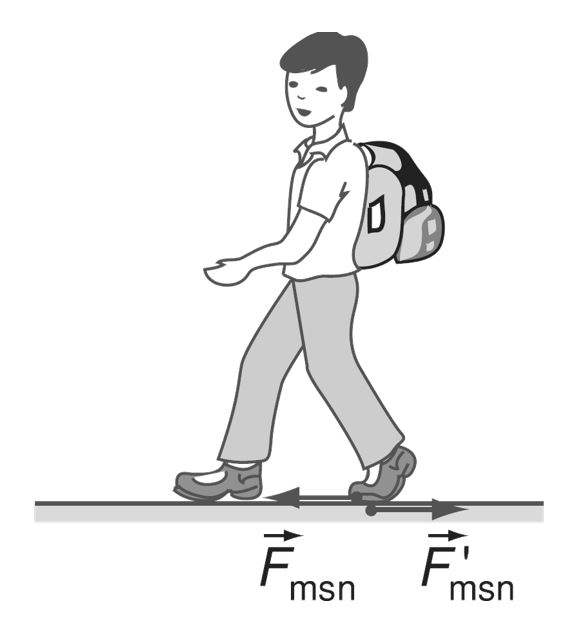
\includegraphics[scale=0.35]{../figs/VN10-PH-15-L-012-1-V2-03.JPG}
		\captionof{figure}{Lực ma sát do mặt đất tác dụng lên chân người khi đi sẽ làm cho người có thể tiến về phía trước.}
	\end{center}
	\item Trong những trường hợp ma sát có lợi, người ta tìm cách tăng tính nhám của các mặt tiếp xúc và tăng áp lực lên mặt tiếp xúc, chẳng hạn thêm các rãnh trên đế giày, bánh xe để tăng ma sát.
\end{itemize}

\section{Mục tiêu bài học - Ví dụ minh họa}
\begin{dang}{Ghi nhớ khái niệm các loại lực ma sát}
	\viduii{1}{Hệ số ma sát trượt
		\begin{mcq}
			\item tỉ lệ thuận với lực ma sát trượt và tỉ lệ nghịch với áp lực. 
			\item phụ thuộc diện tích tiếp xúc và tốc độ của vật.
			\item phụ thuộc vào vật liệu và tình trạng của mặt tiếp xúc. 
			\item phụ thuộc vào áp lực.
		\end{mcq}
	}
	{\hide{
		Hệ số ma sát trượt phụ thuộc vào vật liệu và tình trạng của mặt tiếp xúc   
		
		\textbf{Đáp án: C}.
	}}

	\viduii{1}{Chiều của lực ma sát nghỉ
		\begin{mcq}
			\item  Ngược chiều với vận tốc của vật.
			\item  Ngược chiều với gia tốc của vật.
			\item  Ngược chiều với thành phần ngoại lực song song với mặt tiếp xúc.
			\item  Vuông góc với mặt tiếp xúc.
		\end{mcq}
	}
	{\hide{
		Chiều của lực ma sát nghỉ ngược chiều với thành phần ngoại lực song song với mặt tiếp xúc.
		
		\textbf{Đáp án: C}.
	}}


	\viduii{1}{Phát biểu nào sau đây là đúng khi nói về ma sát
		\begin{mcq}
			\item Lực ma sát lăn cản trở chuyển động của vật này trượt trên vật khác.
			\item Khi vật chuyển động chậm dần, lực ma sát nhỏ hơn lực đẩy.
			\item Lực ma sát lăn nhỏ hơn lực ma sát trượt.
			\item Khi vật chuyển động nhanh dần, lực ma sát lớn hơn lực đẩy.
		\end{mcq}
	}
	{\hide{
		A - sai vì: lực ma sát lăn cản trở chuyển động của vật này lăn trên vật khác
		
		B - sai vì: khi vật chuyển động chậm dần, lực ma sát lớn hơn lực đẩy
		
		C - đúng
		
		D - sai vì: khi vật chuyển động nhanh dần, lực ma sát nhỏ hơn lực đẩy
		
		\textbf{Đáp án: C}.
	}}
\end{dang}
\begin{dang}{Tính độ lớn lực ma sát và các đại lượng\\ trong công thức lực ma sát trượt}
	\viduii{2}{Một ô tô khối lượng 1,5 tấn chuyển động thẳng đều trên đường. Hệ số ma sát lăn giữa bánh xe và mặt đường là 0,08. Tính lực làm cản trở chuyển động của xe trên mặt đường (bỏ qua lực cản không khí).
	}
	{\hide{
		\manatip{Trong trường hợp xe chuyển động do lực đẩy của động cơ, ta xem như lực này có phương song song với mặt đất.}
		
		Lực đẩy song song với mặt ngang, nên phản lực có độ lớn bằng với trọng lực. Lực làm cản trở chuyển động của xe trên mặt đường là lực ma sát
		\begin{equation*}
			F_{\text{ms}} =\mu N = \mu  mg =\SI{0.08}{}\cdot(\SI{1.5e3}{\kilogram})\cdot\SI{9.81}{\meter/\second^{2}}\approx \SI{1177}{N}.
		\end{equation*}
		
		
	}}

	\viduii{2}{Một toa tàu có khối lượng 80 tấn chuyển động thẳng đều dưới tác dụng của lực kéo $F = 6\cdot 10^4\ \text{N}$. Xác định lực ma sát và hệ số ma sát giữa toa tàu với mặt đường
	}
	{\hide{
		Tàu chuyển động thẳng đều nên lực ma sát cân bằng với lực kéo của toa tàu
		\begin{equation*}
			F_{\text{ms}} = F_{\text{k}} = \mu mg.
		\end{equation*}
		Suy ra hệ số ma sát
		\begin{equation*}
			\mu = \dfrac{F_{\text{k}}}{mg} = \text{0,075}.
		\end{equation*} 
	}}

\end{dang}
\begin{dang}{Giải bài toán vật chuyển động trên mặt phẳng ngang có ma sát}
	\viduii{3}{Một ô tô khối lượng 1 tấn, chuyển động trên mặt đường nằm ngang. Hệ số ma sát lăn giữa xe và mặt đường là 0,1. Tính lực kéo của động cơ ô tô trong mỗi trường hợp sau
		
		a) Ô tô chuyển động thẳng đều.
		
		b) Ô tô chuyển động nhanh dần đều với gia tốc $a = \SI{2}{m/s}^2$, lấy $g=\SI{10}{m/s^2}$.
	}
	{\hide{
		\begin{center}
			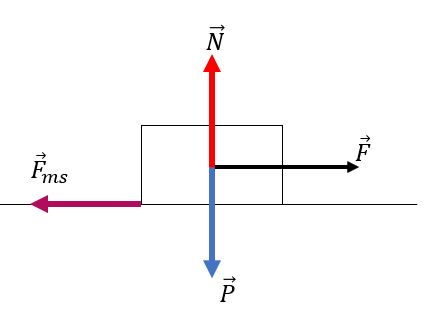
\includegraphics[scale=0.6]{../figs/VN10-PH-15-A-005-3-V2-03.JPG}
		\end{center} 
		Áp dụng định luật II Newton
		\begin{equation*}
			\vec{N}+\vec{P} + \vec{F}_{\text{ms}} + \vec{F} = m\vec{a}.
		\end{equation*}
		Chiếu lên O$y$:
		\begin{equation*}
			N=P = mg.
		\end{equation*}
		Chiếu lên O$x$:
		\begin{equation*}
			F-F_{\text{ms}} = ma \Rightarrow F = ma + F_{\text{ms}}
		\end{equation*}
		a) Khi ô tô chuyển động thẳng đều thì $a=0$ nên lực kéo của ô tô đúng bằng lực ma sát
		\begin{equation*}
			F=F_{\text{ms}} = \mu mg = \SI{1000}{N}.
		\end{equation*}
		b) Khi ô tô chuyển động nhanh dần đều với gia tốc $a = \SI{2}{m/s^2}$ 
		\begin{equation*}
			F= ma + F_{\text{ms}} = ma + \mu mg = m(a+ \mu g) = \SI{3000}{N}.
		\end{equation*}
		
	}}
	
		\viduii{3}{Một ô tô nặng 1,5 tấn chuyển động trên đường nằm ngang chịu tác dụng của lực phát động $\SI{3300}{\newton}$. Ô tô chuyển động với vận tốc đầu $\SI{10}{\meter/\second}$. Sau khi đi $\SI{75}{\meter}$ thì ô tô đạt vận tốc $\SI{72}{\kilo\meter/\hour}$. Lực ma sát giữa ô tô và mặt đường có độ lớn là bao nhiêu?
	}
	{\hide{
		$$\SI{72}{\kilo\meter/\hour}=\SI{2}{\meter/\second}$$
		Chọn chiều dương là chiều chuyển động của ô tô.\\
		Gia tốc của ô tô 
		\begin{equation*}
			v^2-v^2_0 = 2as \Rightarrow a = \dfrac{v^2-v^2_0}{2s} = \SI{2}{m/s^2}.
		\end{equation*}
		Áp dụng định luật II Newton và chiếu lên chiều chuyển động của ô tô:
		\begin{equation*}
			-F_{\text{ms}}+F = ma \Rightarrow F_{\text{ms}} = F-ma = \SI{300}{N}.
		\end{equation*}
		
	}}
	
	\viduii{3}{Một xe lăn, khi được đẩy bằng lực $F = \SI{20}{N}$ nằm ngang thì xe chuyển động thẳng đều. Khi chất lên xe một kiện hàng khối lượng $\SI{20}{kg}$ thì phải chịu tác dụng lực $F = \SI{60}{N}$ nằm ngang xe mới chuyển động thẳng đều. Tính hệ số ma sát giữa xe và mặt dường.
	}
	{\hide{
		Chọn chiều dương là chiều chuyển động của xe.
		
		Khi chưa chất kiện hàng lên xe, xe chuyển động thằng đều nên:
		
		$$\vec P + \vec N + \vec F_\text{ms} + \vec F = \vec 0 \Rightarrow - F_\text{ms} + F =0 \Rightarrow F =F_\text{ms} = \mu mg\ (1).$$
		
		Khi đã chất kiện hàng lên xe, xe chuyển động thẳng đều nên:	
		
		$$\vec P' + \vec N' + \vec F'_\text{ms} + \vec F' = \vec 0 \Rightarrow - F'_\text{ms} + F' =0 \Rightarrow F' =F'_\text{ms} = \mu (m+m_\text{h})g\ (2).$$
		
		Từ (1) và (2) suy ra: 
		
		$$F' - F = \mu g m_\text{h} \Rightarrow \mu =\dfrac{F'-F}{gm_\text{h}} = \SI{0,2}{}.$$
		
		
	}}
	
\end{dang}